\begin{figure*}[t]
  \centering
  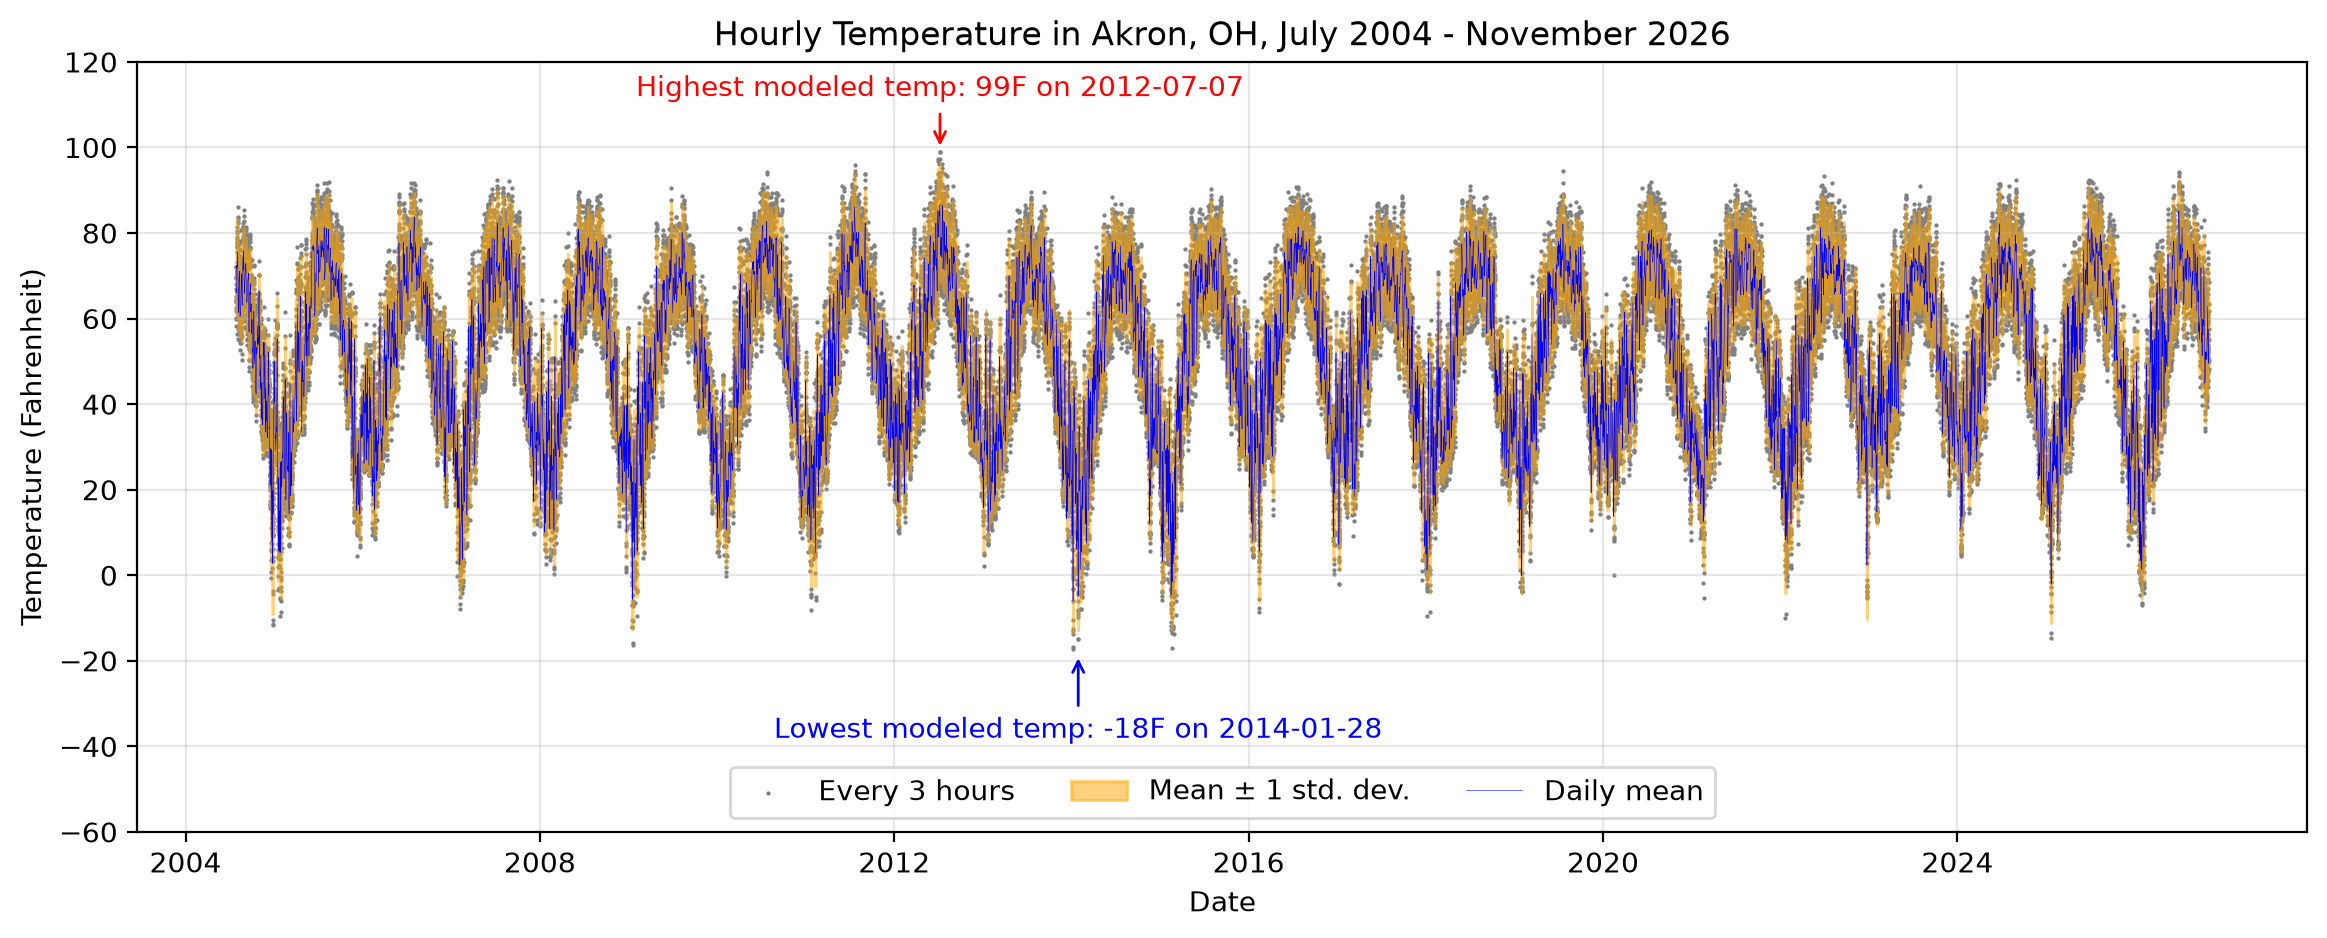
\includegraphics[width=\textwidth,height=0.18\textheight,keepaspectratio]{temperature_full.png}
  \caption{\label{fig:full} Hourly temperature in Akron, OH, July
    2004--November 2026. 
    Gray dots: readings every 3 hours. 
    Blue line:
    daily mean. 
    Orange gradient: daily mean $\pm$ 1 standard deviation.
    Arrows: highest and lowest modeled temperatures.}
\end{figure*}

\begin{figure*}[t]
  \centering
  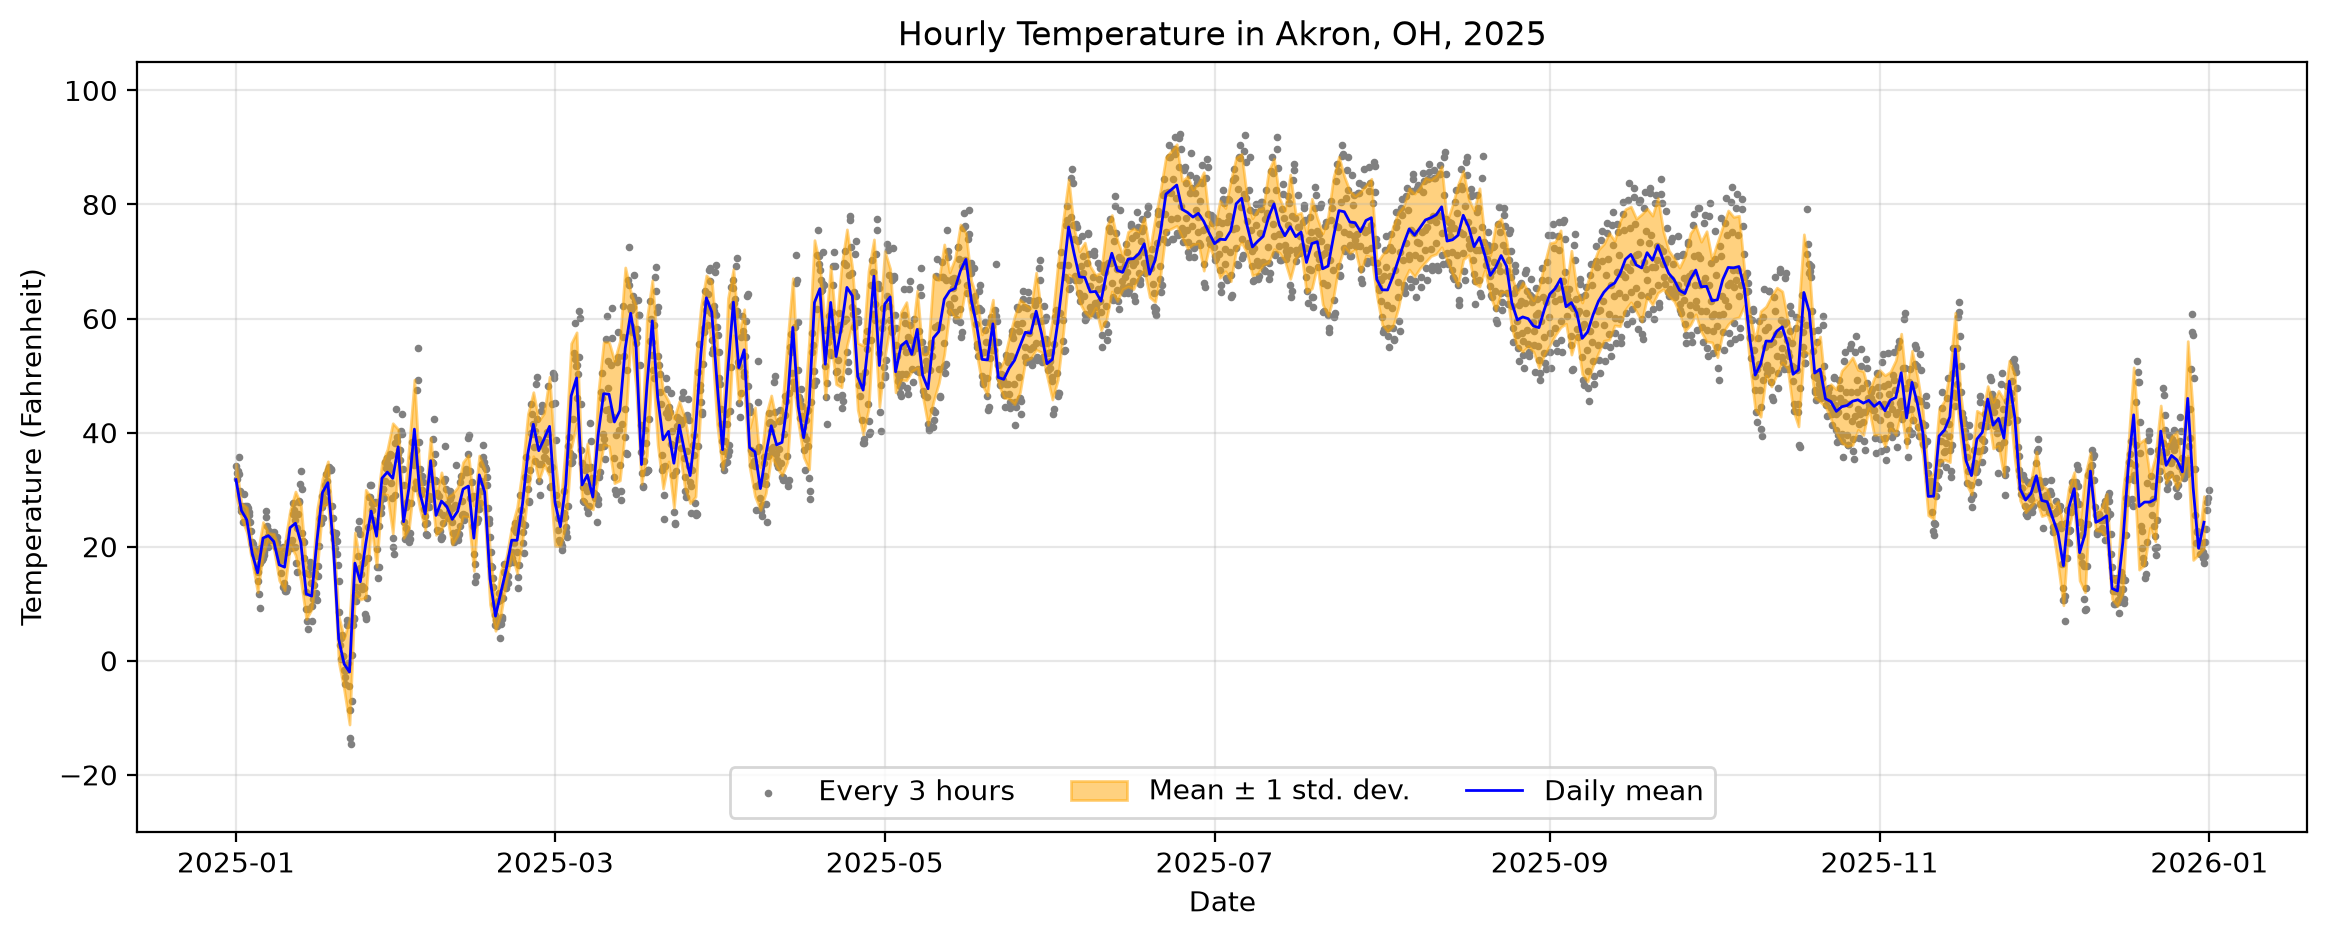
\includegraphics[width=\textwidth,height=0.18\textheight,keepaspectratio]{temperature_2025.png}
  \caption{\label{fig:year} Hourly temperature in Akron, OH, during 2025. 
    Gray dots: readings every 3 hours. 
    Blue line: daily mean. 
    Orange gradient: daily mean $\pm$ 1 standard deviation.}
\end{figure*}

\begin{figure*}[t]
  \centering
  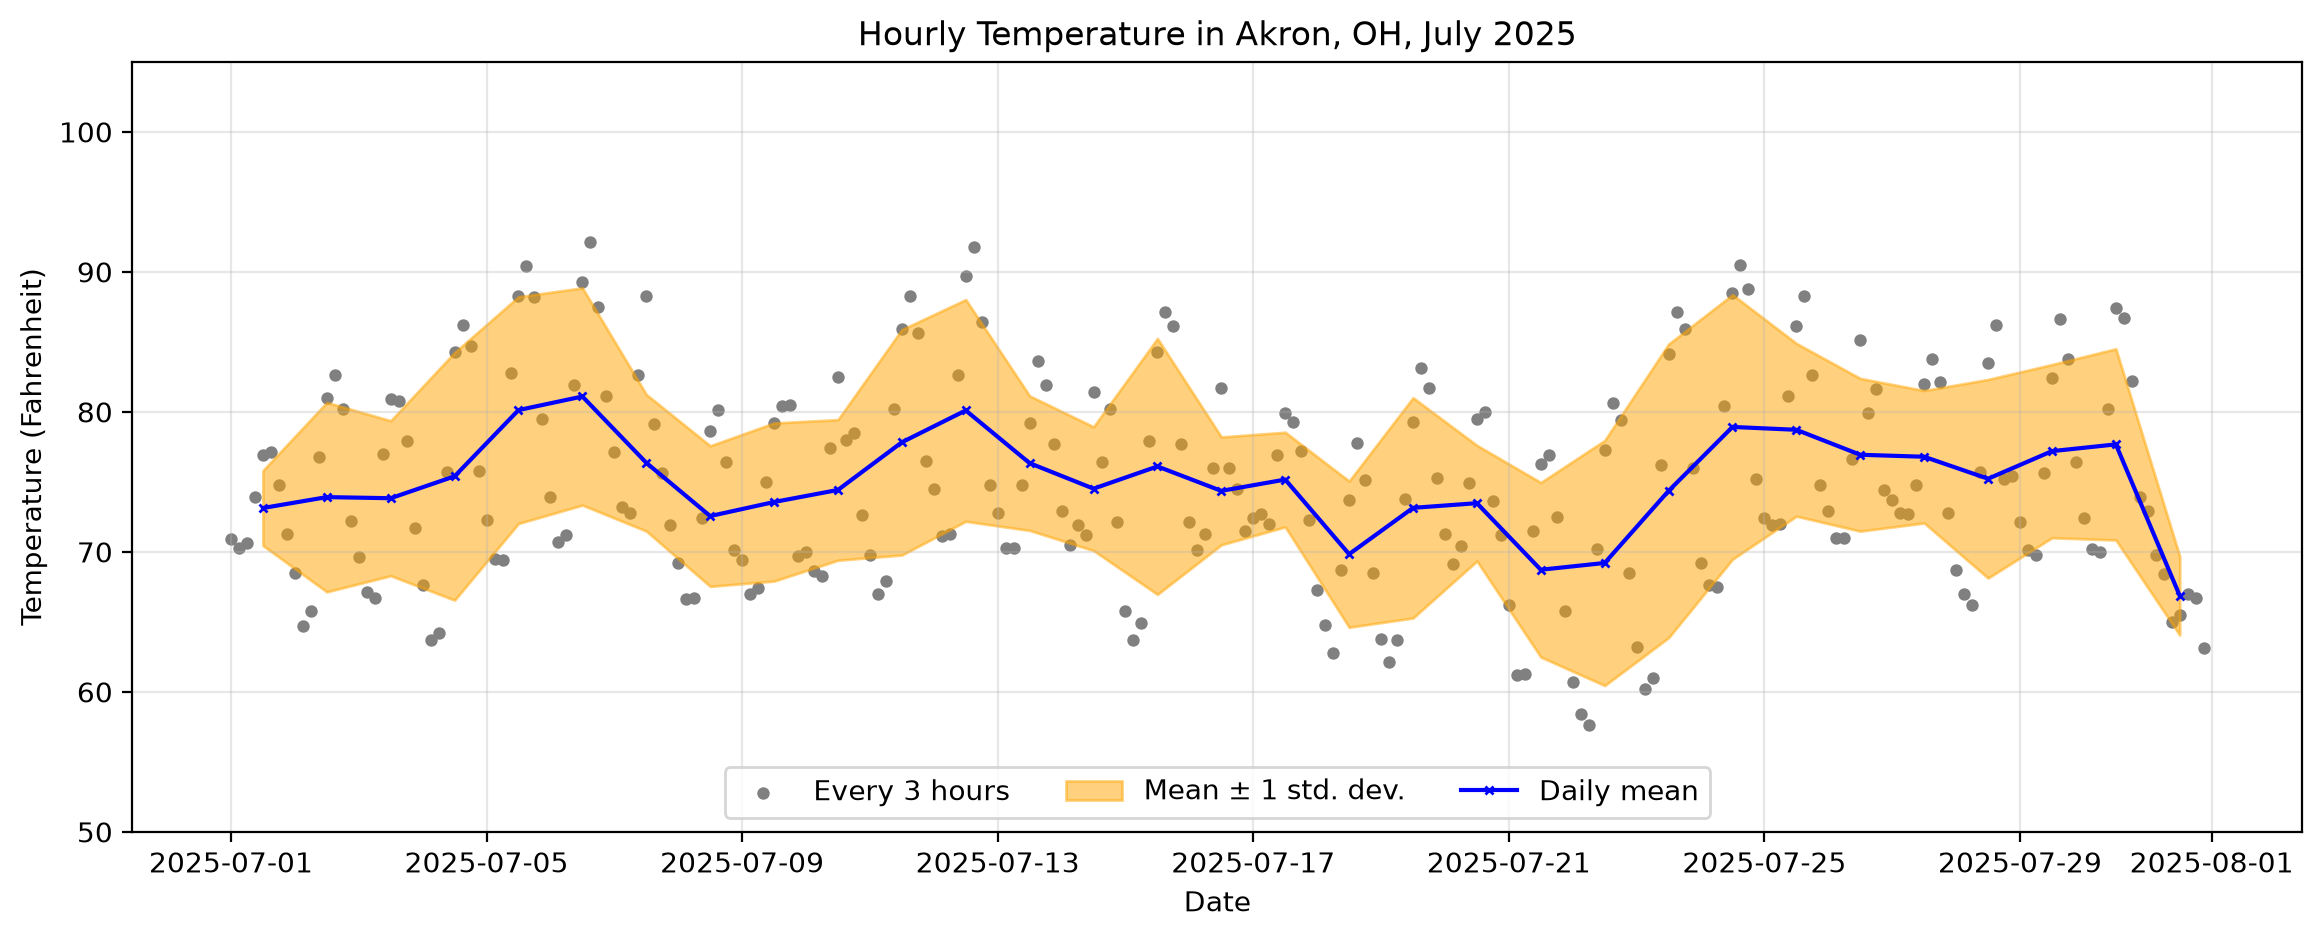
\includegraphics[width=\textwidth,height=0.18\textheight,keepaspectratio]{temperature_month.png}
  \caption{\label{fig:month} Hourly temperature in Akron, OH, during July
    2025.
    Gray dots: readings every 3 hours. 
    Blue line: daily mean. 
    Orange gradient: daily mean $\pm$ 1 standard deviation.}
\end{figure*}

The temperature data was plotted with \texttt{matplotlib}~\cite{hunter07:matplotlib} at three different scales, the full 22 year record, the entire 2025 year, and the entire July 2025 month. In every figure, the gray dots are the raw readings every 3 hours, the blue line is the daily mean (Equation~\ref{eq:mean}), and the orange gradient is the daily mean plus or minus  one standard deviation (Equation~\ref{eq:std}).

Figure~\ref{fig:full} shows the full 22 year record. The seasonal cycle is shown, with the temperature rising to a peak each summer and falling to its lowest point each winter. The provided arrows mark the extremes of the record where the highest modeled temperature was $99$F on July 7, 2012, and the lowest was $-18$F on January 28, 2014. Due to the scale of the graph, individual days are not distinguishable, so Figures~\ref{fig:year} and~\ref{fig:month} show shorter periods.

Figure~\ref{fig:year} shows the entire year of 2025. At this scale, the spread of the gray dots around the daily mean is visible. The daily mean is less stable in the winter and spring then during the summer. In the spring the variation of the temperature would fluctuate, moving 20 degrees within a few days compared to summer where it stays at a consistent 70s.

Figure~\ref{fig:month} zooms in to July 2025. Each day now has its own point on the blue line and its own section of the orange gradient. A tall gradient means a large standard deviation, so the temperature changed a lot that day. A short gradient means the temperature stayed steady. From Figure~\ref{fig:month} we can see that the gradient around July 21--23 was the tallest where temperature went from 60 to 87 over the course of the day.